%preamble - package inclusion and set up
\documentclass[12pt,twoside,a4paper,english]{report} %normal 12pt
% Select encoding of your inputs
\usepackage[utf8]{inputenc}
% Make latex understand and use the typographic
% rules of the language used in the document.
%\usepackage[danish]{babel}
\usepackage[english]{babel}

% Use the vector font Latin Modern which is going
% to be the default font in latex in the future.
%\usepackage{lmodern}
\usepackage{mathptmx}

% Choose the font encoding
\usepackage[T1]{fontenc}

% Use color in tables
\usepackage[table]{xcolor}
\usepackage{pbox}
\usepackage{tabularx}
\usepackage{array}
\usepackage{multirow}

% Load a colour package
\usepackage{xcolor}
\definecolor{aaublue}{RGB}{33,26,82}  %<--define aaublue
\definecolor{white}{RGB}{255,255,255} %<--define white

% ref stuffz			original position
%\usepackage{cleveref}

% The standard graphics inclusion package
\usepackage{graphicx}

\makeatletter
  \g@addto@macro\@floatboxreset\centering %<--centering all figures
\makeatother

\usepackage{adjustbox}

% Set up how figure and table captions are displayed

\usepackage{float}
\restylefloat{figure}
\usepackage{caption}
\usepackage{subfigure}
\usepackage[subfigure]{tocloft}
\captionsetup
{
  %justification = centering,    %<--centering caption with multiple lines
  %justification = raggedright,  %<-- right alings caption with multiple lines
  justification = justified,  %<-- justify alings (make left and right side equal) caption with multiple lines
  font          = footnotesize, %<--set font size to footnotesize
  labelfont     = bf            %<--bold label (e.g., Figure 3.2) font
}
\captionsetup[subfigure]
{
  justification = centering, %<--centering subfigure caption text
  singlelinecheck=false,
  font = footnotesize        %<--font size for subfigures
} 

% Enable row combination in tables
\usepackage{multirow}

% Make space between table lines and text
\renewcommand{\arraystretch}{1.5}

% Enable commands like \st (strike out) and \hl (high light)
\usepackage{soul}

% Make the standard latex tables look so much better
\usepackage{array,booktabs}

% Enable the use of frames around, e.g., theorems
% The framed package is used in the example environment
\usepackage{framed}
\usepackage{colortbl}
\usepackage{longtable}
\usepackage{xcolor}
\usepackage{textcomp}

%-------MATHEMATICS---------------------------------
% Defines new environments such as equation,
% align and split 
\usepackage{amsmath}
\usepackage{relsize}
% Adds new math symbols
\usepackage{amssymb}
% Use theorems in your document
% The ntheorem package is also used for the example environment
% When using thmmarks, amsmath must be an option as well. Otherwise \eqref doesn't work anymore.
\usepackage[framed,amsmath,thmmarks]{ntheorem}
\usepackage{xifthen}%<--enables ifthenelse which is used in macros

\usepackage{siunitx} 
\sisetup{decimalsymbol=period}%<--\num{} will swich commas with periods
\sisetup{detect-weight}
%---------------------------------------------------

%-------PAGE LAYOUT---------------------------------
% Change margins, papersize, etc of the document
\usepackage[
  left=25mm,% left margin on an odd page %tidligere 25mm for baade right og left
  right=25mm,% right margin on an odd page
  top=35mm,
  ]{geometry}
  
% Modify how \chapter, \section, etc. look
% The titlesec package is very configureable
\usepackage{titlesec}
\makeatletter
\def\ttl@mkchap@i#1#2#3#4#5#6#7{%
    \ttl@assign\@tempskipa#3\relax\beforetitleunit
    \vspace{\@tempskipa}%<<<<<< REMOVE THE * AFTER \vspace
    \global\@afterindenttrue
    \ifcase#5 \global\@afterindentfalse\fi
    \ttl@assign\@tempskipb#4\relax\aftertitleunit
    \ttl@topmode{\@tempskipb}{%
        \ttl@select{#6}{#1}{#2}{#7}}%
    \ttl@finmarks  % Outside the box!
    \@ifundefined{ttlp@#6}{}{\ttlp@write{#6}}}
\makeatother

\titlespacing{\chapter}{0pt}{0pt}{10pt}
\titlespacing{\section}{0pt}{0pt}{-5pt}
\titlespacing{\subsection}{0pt}{8pt}{-5pt}
\titlespacing{\subsubsection}{0pt}{6pt}{-10pt}

\titleformat*{\section}{\normalfont\Large\bfseries\color{aaublue}}
\titleformat*{\subsection}{\normalfont\large\bfseries\color{aaublue}}
\titleformat*{\subsubsection}{\normalfont\normalsize\bfseries\color{aaublue}}

\usepackage{titlesec, blindtext, color}
%\color{gray75}{gray}{0.75}
\newcommand{\hsp}{\hspace{20pt}}
\titleformat{\chapter}[hang]{\Huge\bfseries}{\thechapter\hsp\textcolor{aaublue}{|}\hsp}{0pt}{\Huge\bfseries}

% Change the headers and footers
\usepackage{fancyhdr}
\setlength{\headheight}{15pt}
\pagestyle{fancy}
\fancyhf{} %delete everything
\renewcommand{\headrulewidth}{0pt} %remove the horizontal line in the header
\fancyhead[RO,LE]{\color{aaublue}\small\nouppercase\leftmark} %even page - chapter title
\fancyhead[LO]{}
\fancyhead[RE]{} 
\fancyhead[CE]{}
\fancyhead[CO]{}
\fancyfoot[RE,LO]{\thepage}
\fancyfoot[LE,RO]{} %page number on all pages
\fancyfoot[CE,CO]{}

% change first page of all chapters header and footer to fancy style
\makeatletter
\let\ps@plain\ps@fancy
\makeatother

% Do not stretch the content of a page. Instead,
% insert white space at the bottom of the page
\raggedbottom

% Enable arithmetics with length. Useful when typesetting the layout.
\usepackage{calc}
%---------------------------------------------------

\usepackage{appendix}

%-------BIBLIOGRAPHY--------------------------------
%setting references (using numbers) and supporting i.a. Chicargo-style:
\usepackage{etex}
\usepackage{etoolbox}
\usepackage{keyval}
\usepackage{ifthen}
\usepackage{url}
\usepackage{csquotes}
\usepackage[backend=bibtex, isbn=false, url=false, eprint=false, doi=false, style=numeric, sorting=none]{biblatex}
\addbibresource{setup/Canada-Project.bib}
%---------------------------------------------------

%-------MISC----------------------------------------
%%% Enables the use FiXme refferences. Syntax: \fxnote{...} %%%
\usepackage[footnote, draft, english, silent, nomargin]{fixme}		%>>>> draft OR final <<<< 
%With "final" instead of "draft" an error will ocure for every FiXme under compilation.

%%% allows use of lorem ipsum (generate i.e. pagagraph 1 to 5 with \lipsum[1-5]) %%%
\usepackage{lipsum}

%%% Enables figures with text wrapped tightly around it %%%
\usepackage{wrapfig}

%%% Section debth included in table of contents (1 = down to sections) %%%
\setcounter{tocdepth}{1}

%%% Section debth for numbers (1 = down to sections) %%%
\setcounter{secnumdepth}{2}

\usepackage{tocloft}
\setlength{\cftbeforetoctitleskip}{0 cm}
\renewcommand{\cftpartpresnum}{Del~}
\let\cftoldpartfont\cftpartfont
\renewcommand{\cftpartfont}{\cftoldpartfont\cftpartpresnum}
%---------------------------------------------------

%-------DANSK SPROG---------------------------------

%\addto\captionsdanish{%
%	\renewcommand{\figurename}{figur}%
%	\let\figureautorefname\figurename%
%	\renewcommand{\tablename}{tabel}%
%	\let\tableautorefname\tablename%
%%	\renewcommand{\equationname}{ligning}%
%%	\let\equationautorefname\equationname%
%	\renewcommand{\chaptername}{Kapitel}%
%	\let\chapterautorefname\chaptername%
%	\renewcommand{\partname}{Del}%
%	\let\partautorefname\partname%
%	\renewcommand{\sectionname}{afsnit}%
%	\let\sectionautorefname\sectionname%
%%	\renewcommand{\thesubsection}{underafsnit}%
%%	\let\subsectionautorefname\thesubsection%
%	\renewcommand{\pagename}{side}%
%	\let\pageautorefname\pagename%
%}

%-------HYPERLINKS----------------------------------
% Enable hyperlinks and insert info into the pdf
% file. Hypperref should be loaded as one of the 
% last packages
\usepackage{nameref}
\usepackage{hyperref}
\usepackage{bookmark}
\hypersetup{%
	%pdfpagelabels=true,%
	plainpages=false,%
	pdfauthor={Author(s)},%
	pdftitle={Title},%
	pdfsubject={Subject},%
	bookmarksnumbered=true,%
	colorlinks,%
	citecolor=aaublue,%
	filecolor=aaublue,%
	linkcolor=aaublue,% you should probably change this to black before printing
	urlcolor=aaublue,%
	pdfstartview=FitH%
}

% ref stuffz		new position
\usepackage{cleveref}

\crefname{appsec}{bilag}{bilag}
%---------------------------------------------------



% remove all indentations
\setlength\parindent{0pt}
\parskip 5mm
\usepackage{verbatim}

\definecolor{Gra}{RGB}{230,230,230}

%creates a nice-looking C#-text
\newcommand{\CC}{C\nolinebreak\hspace{-.05em}\raisebox{.3ex}{\scriptsize\text \#} }

%enables multi column lists
\usepackage{multicol}

%enables code-examples
\usepackage{listings}

\definecolor{coolblue}{RGB}{32,95,128}
\definecolor{mygreen}{rgb}{0,0.6,0}
\definecolor{mygray}{rgb}{0.5,0.5,0.5}
\definecolor{mymauve}{rgb}{0.58,0,0.82}
\usepackage{textcomp}
\definecolor{listinggray}{gray}{0.9}
\definecolor{lbcolor}{rgb}{0.9,0.9,0.9}

%for c code
\lstdefinestyle{cstyle}{
  backgroundcolor=\color{lbcolor},
	tabsize=4,
	rulecolor=,
	language=C,
  basicstyle=\scriptsize,
  upquote=true,
  aboveskip={1.5\baselineskip},
  columns=fixed,
  showstringspaces=false,
  extendedchars=true,
  breaklines=true,
  prebreak = \raisebox{0ex}[0ex][0ex]{\ensuremath{\hookleftarrow}},
  frame=single,
  showtabs=false,
  numbers=left,
  captionpos=b,
  numbersep=5pt,
  numberstyle=\tiny\color{mygray},
  showspaces=false,
  showstringspaces=false,
  identifierstyle=\ttfamily,
  keywordstyle=\color[rgb]{0,0,1},
  commentstyle=\color[rgb]{0.133,0.545,0.133},
  stringstyle=\color[rgb]{0.627,0.126,0.941},
}
%for python code
\lstdefinestyle{pythonstyle}{
    backgroundcolor=\color{lbcolor},
    tabsize=4,
    rulecolor=,
    language=python,
    basicstyle=\scriptsize,
    upquote=true,
    aboveskip={1.5\baselineskip},
    columns=fixed,
    showstringspaces=false,
    extendedchars=true,
    breaklines=true,
    prebreak = \raisebox{0ex}[0ex][0ex]{\ensuremath{\hookleftarrow}},
    frame=single,
    showtabs=false,
    numbers=left,
    captionpos=b,
    numbersep=5pt,
    numberstyle=\tiny\color{mygray},
    showspaces=false,
    showstringspaces=false,
    identifierstyle=\ttfamily,
    keywordstyle=\color[rgb]{0,0,1},
    commentstyle=\color[rgb]{0.133,0.545,0.133},
    stringstyle=\color[rgb]{0.627,0.126,0.941},
}
%for matlab code
\lstdefinestyle{matlabstyle}{
    backgroundcolor=\color{lbcolor},
    tabsize=4,
    rulecolor=,
    language=Matlab,
    basicstyle=\scriptsize,
    upquote=true,
    aboveskip={1.5\baselineskip},
    columns=fixed,
    showstringspaces=false,
    extendedchars=true,
    breaklines=true,
    prebreak = \raisebox{0ex}[0ex][0ex]{\ensuremath{\hookleftarrow}},
    frame=single,
    showtabs=false,
    numbers=left,
    captionpos=b,
    numbersep=5pt,
    numberstyle=\tiny\color{mygray},
    showspaces=false,
    showstringspaces=false,
    identifierstyle=\ttfamily,
    keywordstyle=\color[rgb]{0,0,1},
    commentstyle=\color[rgb]{0.133,0.545,0.133},
    stringstyle=\color[rgb]{0.627,0.126,0.941},   
}

%for java code
\lstdefinestyle{javastyle}{
	backgroundcolor=\color{lbcolor},
	tabsize=4,
	rulecolor=,
	language=Java,
	basicstyle=\scriptsize,
	upquote=true,
	aboveskip={1.5\baselineskip},
	columns=fixed,
	showstringspaces=false,
	extendedchars=true,
	breaklines=true,
	prebreak = \raisebox{0ex}[0ex][0ex]{\ensuremath{\hookleftarrow}},
	frame=single,
	showtabs=false,
	numbers=left,
	captionpos=b,
	numbersep=5pt,
	numberstyle=\tiny\color{mygray},
	showspaces=false,
	showstringspaces=false,
	identifierstyle=\ttfamily,
	keywordstyle=\color[rgb]{0,0,1},
	commentstyle=\color[rgb]{0.133,0.545,0.133},
	stringstyle=\color[rgb]{0.627,0.126,0.941},
}

%for inline c, syntax: \cline{ codeHere(); }
\lstdefinestyle{cinline}{
    style=cstyle,
    basicstyle=\small,
}
\newcommand\inlinec[1]{ \lstinline[style=cinline]{#1} }

%for inline python, syntax: \pythonline{ codeHere(); }
\lstdefinestyle{pythoninline}{
    style=pythonstyle,
    basicstyle=\small,
}
\newcommand\inlinepython[1]{ \lstinline[style=pythoninline]{#1} }

%for inline matlab, syntax: \matlabline{ codeHere(); }
\lstdefinestyle{matlabinline}{
    style=matlabstyle,
    basicstyle=\small,
}
\newcommand\inlinematlab[1]{ \lstinline[style=matlabinline]{#1} }

\usepackage{enumitem}
%\usepackage[citestyle=authoryear,natbib=true]{biblatex}

% Figures - TIKZ
\usepackage{tikz}
\usepackage[americanresistors,americaninductors,americancurrents, americanvoltages]{circuitikz}

% Wall of text logo
\newcommand{\walloftextalert}[0]{\includegraphics[width=\textwidth]{walloftext.png}}

\usepackage{pdfpages}
\usepackage{lastpage}
\usepackage{epstopdf}

\setlength{\headheight}{21pt}

\hfuzz=\maxdimen
\tolerance = 10000
\hbadness  = 10000

\usepackage{siunitx}
\graphicspath{{./figures/}}

%macros - please read this file
%Macro for 'where'-enviroment was improved by Andrea and Niels :-)

%-----------UNITS-------------------------------------------
\newcommand{\unit}[1]{&& \left[\si{#1}\right]}
%
%\newcommand{\unit}[1]{[\si{#1}]}            %<<| Use these if you want equations to be
%\newcommand{\eq}[2]{&&\si{#1} &= \si{#2}&&} %<<| centered.. .. will appear scrambled
%                                            %  | from one equation to the next though..
%                                            %  | and does not work with long equations.. :/
%
%-----------------------------------------------------------

%-----------WHERE ENVIRONMENT-------------------------------
\newenvironment{where}{\leavevmode{\parindent=1em\indent} Where:\\}{}
\newcommand{\va}[3]
{
  \begin{tabular}{p{20pt} p{40pt} p{290pt} l}
    & { $#1$ } & { #2 } & \ifthenelse{\isempty{ #3 }}  {}  {[{\si{#3}}]} \\
  \end{tabular}\\
}
%-----------------------------------------------------------

%-----------TikZ SETTINGS-----------------------------------
\tikzset{
  block/.style    = {draw, thick, rectangle,
                     minimum height = 2.1em,
                     minimum width = 1.7em},
  sum/.style      = {draw, circle, inner sep=3pt} %<--Adder
}
%-----------------------------------------------------------


%-----------Fanzy reference SETTINGS------------------------
%Figure references:
\newcommand{\figref}[1]{figure \ref{#1}}

%Figure references after full stop/period:
\newcommand{\Figref}[1]{Figure \ref{#1}}

%Table references:
\newcommand{\tabref}[1]{table \ref{#1}}

%Table references after full stop/period:
\newcommand{\Tabref}[1]{Table \ref{#1}}

%Section references:
\newcommand{\secref}[1]{section \ref{#1}} % on page \pageref{#1}}

%Section references:
\newcommand{\Secref}[1]{Section \ref{#1}} % on page \pageref{#1}}

%Subsection references:
\renewcommand{\subref}[1]{section \ref{#1}} % on page \pageref{#1}}

%Subsection references:
\renewcommand{\Subref}[1]{Section \ref{#1}} % on page \pageref{#1}}

%Appendix references:
\newcommand{\appref}[1]{appendix \ref{#1}} % on page \pageref{#1}}

%Appendix references:
\newcommand{\Appref}[1]{Appendix \ref{#1}} % on page \pageref{#1}}

%chapter references: 
\newcommand{\chapref}[1]{chapter \ref{#1}} % on page \pageref{#1}}

%chapter references: 
\newcommand{\Chapref}[1]{Chapter \ref{#1}} % on page \pageref{#1}}

%Units:
%\newcommand{\unit}[1]{&& \left[\si{#1}\right]}

%Text:
\newcommand{\tx}[1]{\text{#1}}

%Equation references:
%1 equation:
\renewcommand{\eqref}[1]{equation (\ref{#1})}

%-----------------------------------------------------------





\begin{document}       % TIP: If you are using TeXstudio you can open
%\tableofcontents      %      the file by Ctrl+LeftClick on setup/macros.tex
%\pagebreak             %      If the file doesn't exist, you will be asked
					   %      weather or not you want to create it.
%\begin{center}
%	\vspace{5cm}
%	\Huge{Worksheets}
%\end{center}
%\clearpage

%||||||||||||||||||||||||||||||||||||||||||||||||||||||||||||||||
%|||||||                 Example Inputs                  ||||||||
%||||||||||||||||||||||||||||||||||||||||||||||||||||||||||||||||
%|||||||                                                 ||||||||
%			 \chapter{Figure Sample}

\begin{figure}[H]                                         %   File-type can be specified
  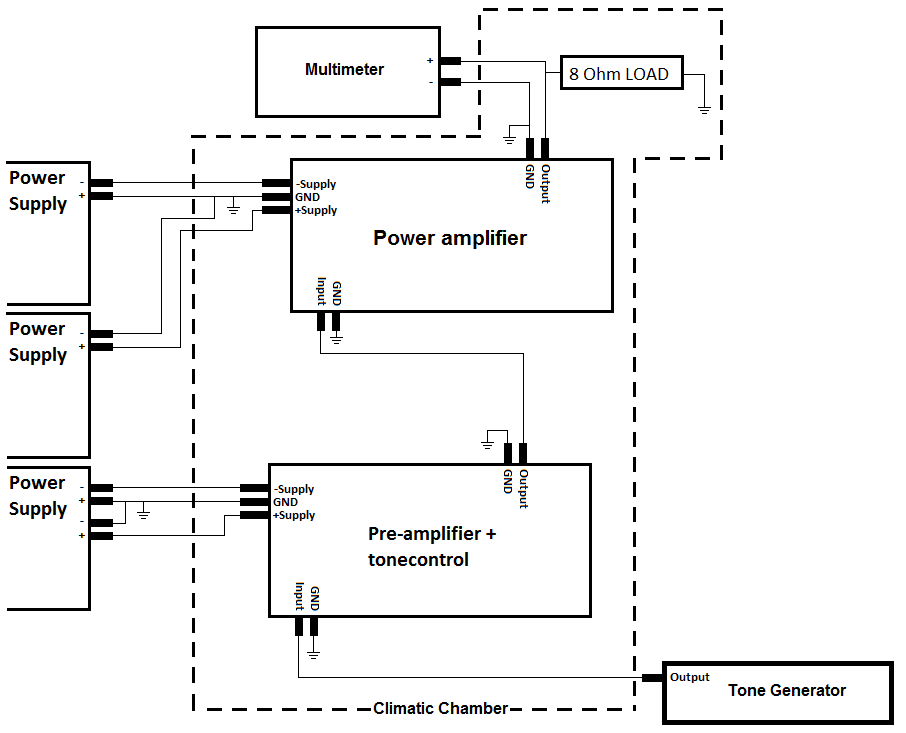
\includegraphics[width=.4\textwidth]{figures/filename}  %<--but is not needed.
  \caption{This image is clearly too small, remember to scale appropriately \fxnote{Remember source}}
  \label{fig:FigureLABEL}  %<--give the figure a label, so you can reference!
\end{figure}               %   For the label to work it must be under the caption.

% Fxnotes will not compile properly inside the figure, only in the caption.
% When \fxnote{} is used in caption, it does not show in a footnote as it normally 
% would, it does however appear in list of corrections.

\autoref{fig:FigureLABEL} $\leftarrow$ use autoref, unless you are referring to multiple pictures, then do like this: \autoref{fig:HbridgeClokwise4Q} and \ref{fig:HbridgeCounterClokwise4Q}.

%Do NOT use \vspace{length}, \hspace{length} or \noindent etc. unless exceedingly necessary - LaTeX is a markup language, let it do its job.
\vspace{.5cm}
\noindent
%
%--------- BIBLIOGRAPHY REF EKSAMPLE -----------------------------------
This reference only represents this line since it is before the punctuation mark\cite{YDing}. This next reference however represents the entire section. That is, all of the preceding sentences in the entire section. This is due to the fact that it is now after the punctuation mark in the end of the section (this is not used in the middle of a section!).\cite{YDing}

%>>PLEASE ALSO READ THE NOTE IN bibliography/bibliography.bib<<

Here is a way to make two images appear on the side of each other. Also, if you modified an image, this is how you properly refer to its original source:

\begin{figure}[H]
    \subcaptionbox  %<--use captionbox instead if no global caption is needed
    {               %                                \%-%-%-%-%-%-%\
      Clockwise 4Q operation.\newline                              %\
      \emph{Edited from image by Biezl.\cite{Biezl}}                %\
      \label{fig:HbridgeClokwise4Q}                                  %\
    }                                                                 %\
    {                                                                  %\
      \includegraphics[width=.46\textwidth]{HbridgeClockwise4Q}         %\
    }                                                                    %\
    \hspace{5pt}                                                          %\
    \subcaptionbox  %<-----------------------------------------------------%\
    {                                                                       %\
      Counterclockwise 4Q operation.\newline                                 %\
      \emph{Edited from image by Biezl.\cite{Biezl}}                          %\
      \label{fig:HbridgeCounterClokwise4Q}                                     %\
    }                                                                           %\
    {                                                                            %\
      \includegraphics[width=.46\textwidth]{HbridgeCounterClockwise4Q}            %|
    }                                                                             %|
    \caption{The 4 quadrant H-bridge configuration shown in both directions.}%<-%-/
    \label{fig:Hbridges}
\end{figure}

As seen \autoref{fig:HbridgeCounterClokwise4Q} can be referred to on its own, or you can use \autoref{fig:Hbridges} to refer to both \autoref{fig:HbridgeClokwise4Q} and \autoref{fig:HbridgeCounterClokwise4Q}.

If the figures are not directly related you might not want to use \textbf{(a)} and \textbf{(b)}, but instead give each figure their own label, here is an example:

\begin{figure}[H]
    \captionbox
    {
      Clockwise 4Q operation.\newline
      \emph{Edited from image by Biezl.\cite{Biezl}}
      \label{fig:HbridgeClokwise4Q2}
    }
    {
      \includegraphics[width=.46\textwidth]{HbridgeClockwise4Q}
    }
    \hspace{5pt}
    \captionbox
    {
      Counterclockwise 4Q operation.\newline
      \emph{Edited from image by Biezl.\cite{Biezl}}
      \label{fig:HbridgeCounterClokwise4Q2}
    }
    {
      \includegraphics[width=.46\textwidth]{HbridgeCounterClockwise4Q}
    }
\end{figure}

In this case \autoref{fig:HbridgeClokwise4Q2} can be referred to without involving \autoref{fig:HbridgeCounterClokwise4Q2}.

\pagebreak			 %|||||||
%			 \section{Table Sample} %to view this sample properly in the code, the screen must be
                       %wide enough, or you have to disable word-wrap in your editor.
\begin{table}[H]
\begin{tabular}{|l|p{5cm}|l|l|l|}
  \hline %-----------------------------------------------------------------------------------
  \textbf{No.} &\textbf{Description} &\textbf{Min} &\textbf{Max} &\textbf{Requirements}    \\
  \hline %-----------------------------------------------------------------------------------
  1            & Some Text           & Some Text   & Some Text   & Some Text               \\
               &                     &             &             & Some More Text          \\
               &                     &             &             & Text Text               \\
               &                     &             &             & Text Text Text          \\
  \hline %-----------------------------------------------------------------------------------
  2            & Some Text           & Some Text   & Some Text   & Some Text               \\
  \hline %-----------------------------------------------------------------------------------
  3            & By specifying the
                 width of a column
                 (|p\{5cm\}|) the
                 cells in that column
                 will not exceed the
                 specified width but         %Extra whitespace is used only for clarity
                 instead expand              %and will not affect the compiled output.
                 downward.
                                     & Some Text           & Some Text   & Some Text       \\
  \hline %-----------------------------------------------------------------------------------
  4            & Some Text           & Some Text   & Some Text   & Some Text               \\
  \hline %-----------------------------------------------------------------------------------
  \multicolumn{2}{|l|}{Some Text}    & \multicolumn{3}{l|}{Some Text}                      \\
  \hline %-----------------------------------------------------------------------------------
  \multicolumn{2}{|l|}{Text Text}    & \multicolumn{3}{l|}{Text = Text}                    \\
  \multicolumn{2}{|l|}{}             & \multicolumn{3}{l|}{Text = Text}                    \\
  \multicolumn{2}{|l|}{}             & \multicolumn{3}{l|}{Text = Text}                    \\
  \multicolumn{2}{|l|}{}             & \multicolumn{3}{l|}{Text = Text}                    \\
  \multicolumn{2}{|l|}{}             & \multicolumn{3}{l|}{Text = Text}                    \\
  \hline %-----------------------------------------------------------------------------------
  \multicolumn{2}{|l|}{Some Text}    & \multicolumn{3}{l|}{Teeeexxtt}                      \\
  \multicolumn{2}{|l|}{}             & \multicolumn{3}{l|}{\LaTeX}                         \\
  \hline %-----------------------------------------------------------------------------------
\end{tabular}
\caption{This Is a Table\label{table:TableLABEL}}
\end{table}

\autoref{table:TableLABEL} $\leftarrow$ use autoref, unless you are referring to multiple tables, then do like this: \autoref{table:TableLABEL} and \ref{table:TableLABEL}.

\pagebreak 		     %|||||||
%			 \section{Equation Sample} %<--In American English all Important Words in
                          %   Headlines are with Big Letters

% \unit is a macro. It uses SI units and aligns all the units neatly :)

\textbf{A normal equation:}
\begin{flalign}
  J_m \cdot \dot{\omega}_m(t) &= \tau_m(t) - B_m \cdot \omega_m(t) - r_m \cdot f_c(t)& \unit{N \cdot m}
  \label{eq:MotorGearNewtonSecLaw}
\end{flalign}
%
\begin{where}
  \va{ J_m               }{is the motor's inertia}                     {kg \cdot m^2}
  \va{ \omega_m(t)       }{is the angular velocity of the motor}       {rad \cdot s^{-1}}
  \va{ \dot{\omega}_m(t) }{is the angular acceleration of the motor}   {rad \cdot s^{-2}}
  \va{ \tau_m(t)         }{is the torque delivered by the motor}       {N \cdot m}
  \va{ B_m               }{is the motor's friction coefficient}        {N \cdot m \cdot s \cdot rad^{-1}}
  \va{ r_m               }{is the radius of the gear, $G_m$}           {m}
  \va{ f_c(t)            }{is the contact force between the two gears} {N}
\end{where}

\textbf{If you need to write something with numbers:} %<--Do not use \textbf{} as headlines, it is bad practice
                                                      %   use instead \chapter{}, \section{}, \subcaption{}, \subsubsection{}
                                                      %   in that order - never a \subsubsection{} directly under a \section{}
\begin{flalign}
  B      &= \num{2,2}\cdot 10^{-6}  \ \si{N\cdot m \cdot rad^{-1} \cdot s}& \label{eq:eq2} \\ %<-- if you want two equations to
  \tau_c &= \num{0.0016}            \ \si{N\cdot m}                       & \label{eq:eq3}    %    allign in one envirenment,
\end{flalign}                                                                              %    remember \\
%using \num{} ensures the same use of decimal point throughout the repport
%should you want to change it, the option is set in the preamble, just change 'period' to 'comma':
%\sisetup{decimalsymbol=period}

\autoref{eq:MotorGearNewtonSecLaw} $\leftarrow$ use autoref, unless you are referring to multiple equations, then do like this: \autoref{eq:eq2} and \ref{eq:eq3}.

\pagebreak		 %|||||||
%			 \section{TikZ Sample}

\textbf{TikZ is only for very patient people, I can recommend Inkscape with textext plugin: \url{https://pav.iki.fi/software/textext/}, difficult to install easy to use, and, if used carefully, nice results.}

%heavily commented example
\input{chapters/tikz/TikZblockDiagramSample.tex}

%way to keep the drawing code in a seperate file
\begin{figure}[H]
	\input{chapters/tikz/smallBlockDiagram.tikz}
	\centering
	\caption{Block diagram}
\end{figure}

%TikZ can also be used for circuits
\input{chapters/tikz/TikZcircuitSample.tex}


\pagebreak            %|||||||
%			 \section{Code Sample}

\begin{lstlisting}[ style=cstyle,
                    caption={C Code}, 
                    label=lst:cExample ]
#include "functions.h"

// Constant matrices
const float L[3] = { -11.0, -12.0, -13.0 };
const float B1[4] = { 0.0, -0.2396, 0.0, 0.2396 };
const float B2[4] = { 0.2396, 0.0, -0.2396, 0.0 };
const float B3[4] = { 0.0377, -0.0377, 0.0377, -0.0377 };
\end{lstlisting}

In \autoref{lst:cExample} is some C-code, and here is some in-line C-code: \inlinec{xTaskCreate();}.

\begin{lstlisting}[ style=pythonstyle,
                    caption={Python Code}, 
                    label=lst:pythonExample ]
# This parses the packets to identify messages and decodes them for the logs
class packetParser():
    def __init__(self,accelfile,gpsfile,measstate,fulllog,plog):
        self.GPS = {0: 'Latitude',
                    1: 'Longtitude',
                    2: 'Velocity'}
        self.IMU = {0: 'AccelerationX',
                    1: 'AccelerationY',
                    2: 'AccelerationZ',
                    3: 'GyroscopeX',
                    4: 'GyroscopeY',
                    5: 'GyroscopeZ',
                    6: 'MagnetometerX',
                    7: 'MagnetometerY',
                    8: 'MagnetometerZ',
                    9: 'Temperature'}
        self.MsgID = {0: self.GPS, 1: self.IMU}
        self.DevID = {0: 'GPS', 1: 'IMU'}
        self.accelburst = [0,0,0,0,0,0,0]
        self.accellog = accelfile
        self.fulllog = fulllog
\end{lstlisting}

In \autoref{lst:pythonExample} is some Python-code, and here is some in-line Python-code:\\ \inlinepython{self.plog.write(str(msgnr))}

\begin{lstlisting}[ style=matlabstyle,
                    caption={Matlab Code}, 
                    label=lst:matlabExample ]
  close all
  clear
  clc
  
  % Parameters
  mx=200;     % [kg] mass + added mass in xb direction
  my=250;     % [kg] mass + added mass in yb direction
  Iz=700;     % [kgm2]
  
  dx=70;      % [kg/s] 
  dy=100;     % [kg/s]
  dyaw=50;    % [kgm2/s]
\end{lstlisting}

In \autoref{lst:cExample}, \ref{lst:pythonExample} and \ref{lst:matlabExample} is some code, and here is some in-line matlab: \inlinematlab{randn(50)}            %|||||||
%|||||||                                                 ||||||||
%||||||||||||||||||||||||||||||||||||||||||||||||||||||||||||||||
%||||||||||||||||||||||||||||||||||||||||||||||||||||||||||||||||


%%% Prereport %%%
		\setlength\cftaftertoctitleskip{2pt}
		\setlength\cftafterloftitleskip{6pt}
		\setlength\cftafterlottitleskip{6pt}
%\selectlanguage{danish}
%\title{Testing the performance of linear regressors using inertial information combined with sEMG to minimize the limb position effect in proportional and simultaneous control of lower arm prosthetics.}

%%% Frontmatter Settings %%%
		\pagestyle{empty} %disable headers and footers
		\pagenumbering{roman} %use roman page numbering in the frontmatter I II...
%		\fancyfoot[RE,LO]{17gr7404} %page number on all pages
%		\fancyfoot[LE,RO]{\thepage}
%		\fancyhead[LE,LO,RE,RO]{}

%%% Introductory Formalities %%%
%\includepdf[pages={1}]{formalities/frontpage.pdf}
			\clearpage
\thispagestyle{empty}

\begin{figure}[H]
	\raggedleft{
	
\includegraphics[width=0.3\textwidth]{setup/aaulogo-en.png} }
	\hspace{4.5cm}
	\raggedright{
	
\includegraphics[width=0.35\textwidth]{setup/RNL.png} }
\end{figure} 

\vspace{3 cm}

\begin{center}
	\begin{Huge}
	%	\textbf{- Status Seminar -}\\
	%	\vspace{2cm}
		\textbf{Developing a wearable system to assess balance during advanced dynamic movements}\\ 
	\end{Huge}
%\vspace{5mm}
%\begin{Large}
%	\textbf{- A pilot study -}\\
%\end{Large}
		\vspace{20 mm}
		\begin{Huge}
		3rd semester Masters, Biomedical Engineering \& Informatics - Autumn $2018$\\
		\vspace{3 mm}
	\end{Huge}
	{\Large Project group: $18$gr$9406$} \\
	\vspace{1cm}
	\large{Simon Bruun and Oliver Thomsen Damsgaard}
\end{center}
\vspace*{\fill}

\begin{center}
	\line(1,0){400}
\end{center}

%\newpage
%
%\large{\textbf{Project period:}\\
%P7, Autumn 2017\\
%01/08/2017 - 20/12/2017\\
%
%\textbf{Project group:}\\
%17gr7404\\} %\fxnote{Input group number}
%
%
%\begin{center}
%	\Large{\textbf{Collaborators:}\\
%		\vspace{1.5cm}
%	\rule{10cm}{1pt}\\
%	Irene Uriarte \\
%	
%	\rule{10cm}{1pt}\\
%	Martin Alexander Garenfeld \\
%	
%	\rule{10cm}{1pt}\\
%	Oliver Thomsen Damsgaard \\
%	
%	\rule{10cm}{1pt}\\
%	Simon Bruun \\}
%\end{center}
%
%
%
%\large{\textbf{Supervisors:}\\
%Strahinja Dosen \\
%Jakob Lund Dideriksen \\
%Lotte N.S. Andreasen Struijk} \\
%\\
\newpage
			% <--- the frontpage
%			\pagestyle{fancy}
%%{\small
\strut\vfill % push the content to the bottom of the page
\noindent Copyright \copyright{} Aalborg University 2015\par
\vspace{0.2cm}

\noindent This report is compiled in \LaTeX, originally developed by Leslie Lamport, based on Donald Knuth's \TeX. The main text is written in \emph{Latin Modern} pt 12, designed by Bogusław Jackowski and Janusz M. Nowacki. 
%The document is compiled via the website \url{www.overleaf.com}, an online collaborative based \LaTeX-editor with instant preview, which enables multiple persons to edit the document simultaneously.
Flowcharts and diagrams are made using Microsoft Visio. 
\clearpage
%			%\begin{document} 
\thispagestyle{empty}
\begin{titlepage}
%\begin{nopagebreak}
{\samepage 

\begin{tabular}{r}
\parbox{\textwidth}{  \raisebox{-15mm}{
\includegraphics[height=3cm]{setup/aaulogo-en.png}}
\hfill \hspace{2cm} \parbox{8cm}{\begin{tabular}{l} %4.90
{\small \textbf{\textcolor{aaublue}{{9\textsuperscript{th} Semester, Masters Project}}}}\\
{\small \textbf{\textcolor{aaublue}{School of Medicine and Health}}}\\
%{\small \textbf{\textcolor{aaublue}{Communication Technologies}}}\\ 
{\small \textbf{\textcolor{aaublue}{Biomedical Engineering and Informatics}}}\\
{\small \textcolor{aaublue}{Fredrik Bajers Vej 7A}} \\
{\small \textcolor{aaublue}{9220 Aalborg}} \\
%{\small \textcolor{aaublue}{\emph{http://www.sict.aau.dk/electronics-and-it}}}
\end{tabular}}}
\end{tabular}}

\begin{tabular}{r}
%\parbox{7cm}{

%\textbf{The effect of limb position on myoelectric prosthetic control using linear regression}
%\\
%\textbf{Theme: Biomedical signals and information}

%\small{
%\\
%}


\parbox{5cm}{


\textbf{Project period:}\\
P7, Autumn 2017\\
01/08/2017 - 20/12/2017\\
   
\textbf{Project group:}\\
17gr7404\\ %\fxnote{Input group number}
  
\textbf{Collaborators:}\\
%\rule{5cm}{1pt}\\
%Irene Uriarte \\
%\rule{5cm}{1pt}\\
%Martin Alexander Garenfeld \\
\rule{5cm}{1pt}\\
Simon Bruun \\
\rule{5cm}{1pt}\\
Oliver Thomsen Damsgaard \\


\textbf{Supervisors:}\\
Strahinja Dosen \\
Jakob Lund Dideriksen \\
Lotte N.S. Andreasen Struijk \\
}\\


\textbf{Pages:} 0\\
\textbf{Appendixes:} b \\
%\textbf{Ekstra:} For projektkode: Se forord\\ %eks. en CD eller USB
\textbf{Completed:} 19/12/2017\\

%\end{tabular}


%\vfill &
%\parbox{1cm}{
  %\vspace{.15cm}
  %\hfill
  
  \begin{tabular}{l}
  %{\textbf{Abstract}}\bigskip \\
  \fbox{
    \parbox{6cm}{\bigskip
     {\vfill{\small \lipsum[15]
%write real thing
     \bigskip}}
     }}
   \end{tabular} }

\end{tabular} %\vspace{1cm}



\centering
\textit{Publication of this report's contents, including source references, may only happen in agreement with the authors.}\\
%\textit{Offentliggørelse af rapportens indhold, med kildeangivelse, må kun ske efter aftale med forfatterne.}\\


%\end{nopagebreak}
\end{titlepage}
%\end{document} 			 % <--- the titlesheet - contains the synopsis!!
%%%% Preface %%%
%			\cleardoublepage
%			\lipsum[15]
%write real thing			 % <--- this is the abstract!!
%%\clearpage
%			\chapter*{Preface}

\lipsum[9]

\pagebreak				% <--- the preface
%

\clearpage
			\pdfbookmark[0]{Table of Contents}{label: tableOfCentents}
			\tableofcontents
			\cleardoublepage


%%% Mainmatter Settings %%%
\pagenumbering{arabic} %use arabic page numbering in the mainmatter
\fancyhf{}
\fancyfoot[C]{\thepage} %\text{ of} \pageref{LastPage}			% ADD LABLE{LASTPAGE} TO LAST PAGE !!
\fancyfoot[RE,LO]{18gr9406}																								   %
\fancyhead[RE,LO]{}																												%% } consider fancyfoots
\fancyhead[RE,LO]{\color{aaublue}\small\nouppercase\leftmark} %even page - chapter title %
\pagestyle{fancy}


%---------------------------INPUTS-------------------------------

%\input{contents/statusText.tex}
%\chapter{Introduction} \label{chap:Introduction}



\chapter{Problem Analysis} \label{chap:PA}

%stroke

\section{Cardiovascular Diseases}

%Short introduction to cvd, stroke and the two subtypes
Cardiovascular diseases (CVD) are the number one cause of death on a world wide scale. In 2015 CVDs was estimated to account for more than 31\% of all deaths globally \cite{whocvd2017}. CVD are a collected term for a number of conditions revolving around diseases to the heart and system of blood vessels. According to the World Health Organisation (WHO) the top two causes of global deaths are the CVDs coronary artery disease and stroke. Of the two, stroke accounted for 10\% of deaths in 2016 \cite{whoMortalityStats2018}.
%something on why we focus on stroke rather than coronary artery disease...?

\subsection{Stroke}
%stroke in numbers and causes /cites: (Hering2016chap7 and 8), Mackay2002, Sharma2017
A stroke is caused by either a blockage or rupture of blood vessels in the brain. As such stroke is divided into two subtypes; ischaemic stroke and haemorrhagic stroke. During an ischaemic stroke a blood vessel in the brain is blocked by blood clots caught in narrow blood vessels. The narrowing of blood vessels are commonly caused by other conditions such as high cholesterol, high blood pressure, unhealthy lifestyle and ageing. If a blood vessel is blocked a part of the brain will be shut off from its blood supply. If not treated within minutes this can cause damage to brain cells in the cut-off area \cite{Mackay2002, Hering2016chap7, InternetStroke2018}.
During an haemorrhagic stroke a blood vessel will rupture and blood will leak inside the brain. Depending on where in the brain the leak occurs the haemorrhagic stroke is either a intracerebral haemorrhage or and subarachnoid haemorrhage, intracerebral being inside the brain and subarachnoid occurring in the space between the brain and the cranium. In both types a rupture and leakage of blood can cause a sudden increase in pressure potentially causing damage to brain cells and can lead to sudden unconsciousness and death. The most common causes are high blood pressure, unhealthy lifestyle, diabetes and ageing \cite{Mackay2002, Hering2016chap8, InternetStroke2018}.

\subsection{Stroke Complications}
%post stroke consequences \cite{Sharma2017}
%outcomes/consequences, damages to balance/coordination of movements /cites: Bhalla2016, Sharma2017
Complications following a stroke are common. In surviving patients 30-96\% have been reported to experience post-stroke complications of both physical and psychological nature. Complications involve recurrent stroke and epileptic seizures, cardiac arrhythmias and failure, infections, problems in gastrointestinal and genitourinary systems, complication of immobility, dementia, pain and depression \cite{Bhalla2016}. %[short version:] Consequences include numerous complications of recurrent stroke, mobility, pain and depression.
Thus, the consequences are many, however this study will focus on complications of mobility. Following a stroke complications related to movement are common. Depending on where in the brain the stroke occurs it can have a variety of outcomes that can affect the patients balance and motor control \cite{Zehr2011}. Up to 38\% of stroke patients have been reported to experience spasticity affecting the performance of dynamic muscle movements such as gait. Spasticity and motor control changes can occur following an upper motor neuron lesion.% \cite{Bhalla2016} %, where part of the brain responsible for motor control or neural pathways above the anterior horn cell of the spinal cord have been damaged. \cite{Bhalla2016} 
Stroke patients are also at a higher risk of osteoporosis due to weakening of performing voluntary movements or movements as a whole if the patient experience hemiparesis \cite{Bhalla2016,Zehr2011}.

%spinal cord injury

\section{Spinal Cord Injury}

The spinal cord (SC) is part of the central nervous system (CNS) together with the brain. The SC is connecting the brain to the rest of the body by connecting to the peripheral nervous system (PNS). It is responsible for leading nerve impulses between the brain and body, to modulate movements, sensory inputs and visceral innervation. The SC extends from the brain just below the cranium down the spine to the lumbar vertebrae one and two (L1-L2). From L1-L2 to the end of the spine at the coccyx vertebrae or tailbone, bundles of nerve fibres extend further. The vertebrae bones encapsulates and protects the SC. However, trauma to the spine can cause trauma to the SC as well. \cite{Weidner2017}

The incidence for spinal cord injuries (SCI) ranges from 15 to 39 million a year in industrialized countries. Most traumatic causes are a result of traffic accidents, falls and violence. Causes for non-traumatic SCI are degenerative diseases and tumours. In prevalence of traumatic SCI, men outnumber women at a ratio of 3:1, while the prevalence is near equal in non-traumatic SCI. Any injury to the SC causing neurological damage can lead to serious dysfunction depending on where the injury happens. This can lead to loss of sensory sensation and motor control and dysfunction to bladder, bowel and cardiovascular functions. \cite{Weidner2017}

%loss of motor function lead to bad balance and poor performance of movements. this is bad for patients
%assuming we have eralier in the report specified that we are focusing on movements, balanace and such
According to the National Spinal Cord Injury Statistical Center (NSCISC), the most frequent category for neurological damage is incomplete quadriplegia at $32.2\%$ of cases. This is followed by complete paraplegia at $24.2\%$. Out of all SCI cases only $7.4\%$ reach neurological recovery. \cite{NSCISC2017} %The NSCISC report included 32.727 cases
Many SCI patients experience rehospitalization, depression and pain, following the injury. According to the NSCISC many patients are unsatisfied with their life in the years after injury. However, life satisfaction generally increase with years post injury. \cite{NSCISC2017}
%this is rehab
\section{Rehabilitation}

Patients suffering from neural damage caused by stroke or SCI will in many cases need to go through a rehabilitation process to regain or relearn lost functions \cite{Sandrini2018,Michael2005}. Currently many different methods for rehabilitation exist, many with focus on patients regaining the ability to control their limbs and balance, as a step toward regaining independence. An important aspect of rehabilitation is that when assigning training to patients of SCI or stroke, it is important to evaluate the state of the patient, as different patients will have different levels of dysfunction depending on the severity of the damage caused by SCI or stroke. Rehabilitation should be suited to each patient individually. \cite{Sandrini2018}

\subsection{Current stroke rehabilitation methods}

Gait and balance rehabilitation of stroke patients focus on implementing the locomotion mechanisms, but also the brain, to achieve functional gait on various surfaces. Several studies have indirectly shown that cortical functions are involved in the gait cycle, where they are responsible for reacting and adapting the gait to uneven surfaces. \cite{Belda2011} \\
As in cases of SCI, stroke rehabilitation also focuses on regaining the ability to walk, and therefore the rehabilitation process implements gait training. Stroke patients have the same possibility to exploit motor plasticity, in order to relearn previously known skills. \cite{Belda2011} \\
There are many approaches to gait rehabilitation, where the most relevant in this case is the motor learning techniques. This method gives the patient an active role in the rehabilitation process, and there are multiple approved approaches within this technique. The overall thought behind this technique is to learn new and improve current skills by repetition of specific tasks and utilizing sensory feedback to achieve manipulation of the involved neural systems. \cite{Belda2011}

\subsection{Current SCI rehabilitation methods}

The aim of rehabilitating patients suffering from either stroke or SCI, is to compensate for the abilities they have lost by training the intact parts of their sensory-motor (SM) system. This can be achieved by activating the intact parts of the SM system with sensory cues recruiting both spinal and supra spinal connections. \cite{Sandrini2018}\\
This approach has been shown to work in animal studies, where neural systems in the spinal cord responsible for locomotion were trained independently of the connection to the brain. These methods have been used as the foundation for the current training protocols to train functional movements such as walking in patients with incomplete SCI, meaning the training should make use of the neural plasticity. \cite{Sandrini2018}\\
Training the walking ability includes a treadmill on which the patient will attempt to walk while being supported by an unloading harness. The treadmill walking should activate locomotion movements through the input from load and stretch sensitive mechanoreceptors, resulting in improved coordination, speed and strength. This training method can consist of both explicit and implicit methods, where patients will either receive visual feedback to adjust the length of their steps in order to activate a cognitive process to adjust their gait. The implicit method will rely on resistance in order to train locomotion without the patient having to plan their step length. Another important aspect of rehabilitation of these individuals is their balance, and lately training of this ability has been shown to increase both speed and distance in walking tests. \cite{Sandrini2018}

% Balance and gait training have been moved to own .tex file


%2. Assesment of gait disorders in neurorehabilitation page 69:
%https://link-springer-com.zorac.aub.aau.dk/content/pdf/10.1007%2F978-3-319-72736-3.pdf 
%
%Something about rehabilitation, balance confidence and stability w. multimodal self administered balance training: 3. https://www.ncbi.nlm.nih.gov/pmc/articles/PMC5119910/ 
%and with strength training: 4. https://www.ncbi.nlm.nih.gov/pmc/articles/PMC3885846/ 
%
%Something about the balance over the course of acute rehabilitation: 5. https://www.archives-pmr.org/article/S0003-9993(95)81035-8/abstract
%
%7. Accelerometer mounted on people: http://iopscience.iop.org/article/10.1088/0967-3334/37/10/1785
%
%8. Something with peoples activity when they have had a stroke: https://www.sciencedirect.com/science/article/pii/S0003999305001905
%
%9. Stroke rehab guidelines: http://journals.sagepub.com/doi/pdf/10.1177/1747493016643553
%
%10. SCI guidelines side 227, measuring side 238, appropriate outcome measures side 76, stroke 187 https://link-springer-com.zorac.aub.aau.dk/content/pdf/10.1007%2F978-3-319-72736-3.pdf
%
%11. Stroke Rehab:
%https://jneuroengrehab.biomedcentral.com/articles/10.1186/1743-0003-8-66
%
%12. New methods for gait analysis page 235:
%https://link-springer-com.zorac.aub.aau.dk/content/pdf/10.1007%2F978-3-319-72736-3.pdf
%
%13. Something with Tai Chi:
%https://journals.lww.com/ajpmr/FullText/2012/12000/Tai_Chi_for_Stroke_Rehabilitation__A_Focused.10.aspx 
%
%14. Something with dual-task vs. single-task:
%http://journals.sagepub.com/doi/full/10.1177/0269215518758482
%
%15. More on tai chi:
%http://journals.sagepub.com/doi/full/10.1177/0269215518773442
%
%16. Pilates:
%https://journals.humankinetics.com/doi/full/10.1123/japa.2017-0078
%
%What we want is to measure reliance on walking device plus activity patterns.
%section on outcome measures used to assess patients physical functionality and the rehabilitation progress.
\section{Assessing gait in rehabilitation}

It is common for rehabilitation programs to focus on patients regaining their ability to walk following impairment of movement due to stroke or SCI. Walking is an important part of life and is a large factor for autonomy and independence in daily life. 
Several different methods for assessing patient gait abilities have been developed to evaluate on the rehabilitation progress. Many of these outcome measures are also used in studies on the development of new technologies and methods. According to the Italian Robotic Neurorehabilitation Research Group (IRNRG) there are six outcome measures which are used more commonly in research studies. These six are: Functional Ambulation Category (FAC), the 10-m Walking Test, the Motricity Index, the 6-Minute Walking Test, the Rivermead Mobility Index and the Berg Balance Scale (BBS). \cite{Sandrini2018}

\subsection{Measuring Gait In a Clinical Environment}

Recent technological improvements makes it possible to perform advanced gait analysis (GA) while examining 3D kinematics and EMG in a clinical setting. This method provides the clinician with an advanced insight in the patients current abilities and gives the possibility of measuring and quantizing any changes that might occur during a rehabilitation process. \cite{Sandrini2018}

The method of using 3D kinematics takes place in a laboratory with the use of cameras, surface electromyography (sEMG), force platforms and stereophotogrammetry equipment to provide the needed data to perform GA. The system provides recordings for qualitative analysis, as well as quantitative measures of muscle activation, contact forces with the ground and body position during gait. These measures are used to evaluate the gait cycle with regards to step length, cadence, swing time, rotation and power in the joints for the individual subject. \cite{Sandrini2018}\\
An attempt to quantify the quality of gait with a single parameter was made with the Normalcy Index (NI), where the algorithm measures deviation of a patients gait pattern from the gait of healthy individuals through Principal Component Analysis (PCA). The mean pattern is based on some of the features obtained with GA. This method has been proven to be an effective tool to examine changes in gait over time. \cite{Sandrini2018}
Further advances in the quantification of the many features is the gait deviation index, the gait profile score and the movement deviation profile. All of these methods take different approaches to finding the deviation between healthy gait and the measured variables from the advanced clinical set-up described briefly above. \cite{Sandrini2018}\\
Other approaches exist to measure improvement during rehabilitation. One study calculated the combined centre of pressure of the patient and a walking frame (WF) as a combined system, by measuring reaction forces of both the patient and the WF along with cameras capturing the placement of the feet relative to the WF. This gave the possibility to calculate the weight supported through the frame and the stability of both patient and WF. \cite{Costamagna2017}

\subsection{Measuring Gait Outside a Clinical Environment}

Methods of measuring gait and other dynamic activities outside clinical environments are becoming more accessible and favourable over measurement methods bound to clinical environments. Rehabilitation and assessment in clinical environments rarely translate well to real life situations \cite{Basteris2014}. Such systems are most functional if they are wearable by the patient or test subject. 

Wearable systems to analyse and monitor body dynamics are attracting an increased interest in research, where accelerometers and inertial measurement units (IMU) are the most used in newer studies. Here, studies have used wearable systems to measure upper limb kinematics and trunk posture, to evaluate on movement performance. \cite{Wang2017} Wearable systems can also be used for assessing gait by implementing multiple sensors placed on the subjects lower limbs, measuring variables such as acceleration, gyroscopic, pressure forces and EMG depending on which system is implemented. Here, measuring forces applied to the feet can be done with simple force sensors based on either resistive, piezoelectric or capacitive designs, and often includes an implementation of these in shoes or insoles. \cite{Muro2014} A study by Muro et al. \cite{Muro2014} has been shown that the implementation into insoles reflects the measurements obtained from clinical motion analysis laboratories. \\
Inertial measurement units (IMU) can also be implemented in wearable devices. These consist of gyroscopes measuring the rotational inertia used to measure changes in direction, as well as accelerometers measuring the acceleration in three axes giving the opportunity to measure changes in balance or sudden knocks such as those experienced by the sensor while walking. \cite{Muro2014}

A study by Hurwitz et al. \cite{Hurwitz2016}, examined the importance of accelerometer position, age and walking speed on the accuracy of accelerometer based measurement of gait. It was found that the device location did not affect measures such as speed, cadence and single limb support time. Gait asymmetry and variability was shown to be affected by age and walking speed. 


%NOT USED ANYMERE
%This study aims to measure improvement of reliance on a WF outside the clinical setting, as well as change in activity in everyday life based on a simple system with inspiration from what was developed in \cite{Costamanga2017} and \cite{Hurwitz2016}. The outcome measures that should be achieved with the system is stability, reliance on WF based on the weight distribution between the patient and the WF, number of steps taken as well as an overview of the daily activity of the patients before, during and after rehabilitation.
% det er ikke længere det vi gør

%\subsection{Wearable Systems Used in Gait Assessment}

%Wearable systems for gait assessment implements multiple sensors placed on the subject, measuring variables such as acceleration, gyroscopic and pressure forces and EMG depending on what system is implemented. \cite{Muro2014}

%Measuring forces applied to the feet can be done with simple force sensors based on either resistive, piezoelectric or capacitive designs, and often includes an implementation of these in shoes or insoles. A study by Muro et al. \cite{Muro2014} has been shown that the implementation into insoles reflects the measurements obtained from clinical motion analysis laboratories. 

%Inertial measurement units (IMU) can also be implemented in wearable devices. These consist of gyroscopes measuring the rotational inertia used to measure changes in direction, as well as accelerometers measuring the acceleration in three axes giving the opportunity to measure changes in balance or sudden knocks such as those experienced by the sensor while walking. \cite{Muro2014}



%The FAC is a method of categorizing patients into six levels depending on the patients ability to walk unaided. The categories range from the patient being able to walk anywhere unaided to the patient not being able to walk at all. Steps of gradually needing more support to be able to walk exist between to the extremes. \cite{Sandrini2018}  

%The 10 meter walking test (10mWT) is a simple test of measuring the time it takes a subject to walk 10 meters. Either steps can be counted or time can be measured
%%no need to describe the tests. 





%following assessing gait in rehab
%current methods of evaluating gait ability -> both inside and outside clinical environments focus on simple movements tasks -> they are non-standardised, and evaluation is based on physicians personal experience -> new method needed: our problem definition

\subsection{Current stroke rehabilitation (and its shortcomings)}
Loosing functionality of mobility can lead to several different risks for the patient, one of which is falls. Both stroke and SCI patients experience a greater risk of falls. The prevention of patients falling should be prioritized as falls can lead to loss of independence and serious injury. Despite the consequences, studies have shown that 30-39\% of stroke patients fall at least once during a rehabilitative process, and of these patients 42\% experience multiple falls. \cite{Bhalla2016, Hanger2014} According to a study by Wannapakhe et. al \cite{Wannapakhe2015}, out of a group of 100 SCI patients, 45 experienced falls during a six month period post rehabilitation. 
Apart from the immediate risks and dangers to patients falling, falls can also further extend the rehabilitation period and worsen the rehabilitation of both motor and cognitive functions \cite{Wong2016, Blennerhassett2012}. This is a problem since strength recovery is usually greatest in the first 100 days following injury \cite{Weidner2017}. 
Current rehabilitation programs still use qualitative methods for evaluating patients progress. These methods rely on the physician to evaluate how well the patient performs \cite{ANPT_SCI2018, ANPT_Stroke2018}. This is a problem since qualitative evaluations are prone to changes from session to session depending on many factors which are not accounted for, like the patients level of energy or the physicians personal experience. 

 

Current ambulatory care does not facilitate high activity levels for patients. A study by Kathleen et al. \cite{Michael2005} have shown patients to have extremely low levels of daily activity (avg. 2837 steps/day) when compared to the norm (5000-6000 steps/day) for sedentary elderly people (65-70 years). Without adequate training and activity patients have little chance of regaining lost mobility, which are as previously described can lead to loss of confidence in performing movements, loss of independence, prolonged rehabilitation period and an increased risk of falls and injury. 


section 4.4.1 in book: neurological aspects of SCI 
- time course of clinical nd functional adaptations
	- motor and functional recovery



%following section describes current inside and outside clinical environment rehab methods, which are already described in cAssessingGait.tex
%Current rehabilitation often involves gait treadmill training for rehabilitating dynamic movements /cite{simons kilde 8}}. However, as often is with training of patients in clinical environments, this approach translates poorly to real life outside the clinical environment \cite{Basteris2014}. In daily life sudden changes in walking speed or change of direction is normal and necessary, however this is often not accounted for on a treadmill in a clinical environment. To improve muscle strength of patients, weights or cables have been used to apply resistance to leg movement when walking on a treadmill, however this approach is cumbersome and cannot be used outside clinical environments. 
%Different methods have been researched to explore ways to both train balance and strength in patients gait. A study by Washabaugh et al. \cite{Washabaugh2016}, developed a device which could be worn outside clinical environments to put resistance on leg movements by applying resistant force at the knee joint. The study showed a significant increase in muscle activity during gait with applied resistance \cite{Washabaugh2016}. Other studies have used assistive robotic devices in gait training. Chisari et al. \cite{Chisari2015} used an assistive robotic device to show significant improvements in hemiparetic patients walking ability, but not in leg muscle strength. Motor imaging training have also been shown to significantly improve on patients gait and leg muscle strength \cite{Kuma2015}. 



%something on that most studies only focus/use treadmill trianing and dont do much in strength training eventhough this is very important. -> this can lead to why we like to do multimodal training which can incorporate both balance AND strength training. 

%kilde 1: Individualized Treadmill and Strength Training for Chronic Stroke Rehabilitation: Effects of Imbalance (søgt adgang hos AUB)
		%study investigate effect of treadmill-strength training. 

%more on the (hopefully) proven/significant worsening of patient performance in balance/gait/dynamic movement following falls compared to non-fallers. [THIS STUDY IS NOT ON FALLS]

%people get stroke -> stroke lead to bad balance and movement -> people fall -> falls are bad -> current rehab does not make patients not fall -> new rehab -> need new evaluation method -> our project

%it would be nice to put patients through a rehabilitation program which effectively increase their balance and performance of dynamic movements. therefore it is necessary to be able to evaluate if patients get better balance/movement






\subsection{New Methods for Balance and Gait Training}
%this section could go before badnessOfCurrentRehab.tex so that badnessOfCurrentRehab is right before the Problemdifinition.tex

% more focus on dual task training to lead to training with advanced dynamic movements like karate/tai chi
In contrast to current rehabilitation methods, mainly focusing on simple gait training, a rhythmic movement, newer approaches have begun to use dual-task training, incorporating cognitive tasks as well. Similarly, training involving advanced movements have suggested to improve balance for both stroke and Parkinson's disease patients \cite{Ding2012,Winser2018}. 

Studies have shown that dual-task mobility training helps improve balance and gait compared to groups that performed single-task training in stroke patients. The dual-task approach was designed to make the patient walk on a treadmill while performing either a cognitive or motor task at the same time. \cite{He2018}
The walking/motor dual-task method proved to be significantly better at improving speed, stride length and cadence for both dual-task and single-task tests. Combining walking and cognitive tasks improved the patients cadence and dynamic gait index, which describes balance while walking, in single-task tests. It was also found that combining balance and cognitive or motor tasks improved a number of balance measures significantly compared to single-task training. \cite{He2018}
Despite the outcomes reported in \cite{He2018}, the conclusion is that more studies are needed in order to support that dual-task training improves performance in dual-task tests. The review study shows that a dual-task approach improves single-task tests compared to the single-task training. \cite{He2018}

A similar approach can be seen in studies where Tai Chi was used as a rehabilitation method for stroke and Parkinson's disease patients, implementing the aspect of thought and simultaneous movement into the training \cite{Ding2012,Winser2018}. This use of martial arts training resulted in multiple studies finding significantly higher improvement in balance compared to the control groups, while gait measures did not improve significantly with the implementation of Tai Chi training. \cite{Ding2012}
These findings can not lead to a final conclusion due to the number of trials and sample size, but the results indicate that martial arts could help increase balance in stroke patients \cite{Ding2012}. It was also found that Tai Chi helps to reduce the number of falls for people suffering from balance problems after both stroke and Parkinson's disease, while in this study it did not result in a significant difference between balance measures compared with regular treatment \cite{Winser2018}. It has also been found that Pilates training improves both static and dynamic balance in older adults compared to the control group that only did their normal daily activities \cite{Moreno2017}.
%problemformuleringsafsnit
\section{Problem definition}

Following the previous chapter the work leads us from the problem of patients suffering from complication of mobility caused by stroke or SCI, to the current rehabilitating methods used to train patients to regain mobility. 
%% this section should be made clear in badnessOfCurrentRehab.tex
However, these methods are not standardised and evaluations of patient performance is subjected to physicians personal experience and patients immediate feeling. Additionally, most evaluations occur in clinical environments when performing simple movement tasks, which translate poorly to real life. 
%%-------------------

It can be discussed whether or not current rehabilitation training with single-task training of simple movements is properly prepares patients to live independent daily lives post rehabilitation. This project propose that training involving advanced dynamic movements can further improve on patients strength and balance, better preparing them for daily life, when compared to traditional simple movement training. 
However, there exist no suitable system to evaluate advanced dynamic movements. Thus a new system is needed to have a way to measure and assess patients ability to perform advanced dynamic movements to determine if this type of training is better than that currently used in rehabilitation. 

%Thus a new method or system is needed to have a standardised and easily assessed method to frequently measure patient improvement for advanced movements in mobility rehabilitation.

\begin{center}
How is it possible to develop a wearable system to measure performance of advanced dynamic movements to evaluate a subjects performance in relation to balance, coordination and sequence of execution.

How is to possible to develop a wearable system to evaluate subjects Centre of Pressure when performing advanced dynamic movements.

Evaluating Centre of Pressure/Balance in subjects performing the karate kata Pinan Nidan. A proof of concept study. 
\end{center}

%\section{Future works}

The future works of the project will focus on measuring balance with a wearable system during advanced movements (Pinan Nidan kata sequence in this case). Our supervisor at UVic would like to quantify improvement of coordination and balance during advanced movements in relation to rehabilitation of balance after stroke or SCI. This leads to our current problem. 

\textit{Is it possible to develop a wearable system to measure balance and coordination during advanced movements in relation to rehabilitation?}

\subsection{Methods}

The system we are most likely to end up with will be a combination of IMU's placed on different parts of the body as well as sensors in the soles to measure centre of pressure during the sequence. The aim is to measure the rotational forces and use these to quantify the coordination of different limb movements, as well as using them to separate the different movements of the sequence. Pressure sensors in the soles will be used to quantify the body sway and thereby the balance in between these movements, where the subjects should be standing in a stable position with weight on both feet. 

We are most likely going to use FlexiForce sensors for the soles along with an amplifier and data logger. The IMU's will be Consensys Shimmers as these are easy to set up and test on different sites of the body. As the movements within the sequence should start at the head going down through the body, we are expecting to place sensors at the top of the neck, on the back, at the hips and on the calves. 

To evaluate the system we will perform tests on both trained and untrained subjects, as well as measuring the change in coordination and balance in untrained subjects over multiple days of training. In the future this could be used by our supervisor to analyse the improvement of balance during advanced, non-locomotor-movements in stroke and SCI patients, as he wants to examine if focusing more on advanced movements during rehabilitation could lead to higher functionality and balance. 


\chapter{Methods} \label{chap:Methods}
%\section{Experiment Protocol / description} %protokol er ikke det rigtige ord

%this will act as the initil part of the methods section. as a header for the chapter

For this project reaction and pressure forces were collected from subjects performing the karate kata Pinan Nidan. %Reaction forces are measured from the subjects body rotations and movements, while pressure forces are measured from under the subjects feet. 
A karate kata is a sequence of detailed choreographed patterns of movements. Many different types of kata exist, each practice visualisation, balance and basic technique through repetition of movements. Different katas have different sequences of movements, some are more difficult than others where jumps and kicks are part of the movements. For this projects data acquisition the kata Pinan Nidan is chosen. 
Pinan Nidan consists of a series of movements involving steps, turning and hand strikes, where the performers' feet are on the ground at most times. Pinan Nidan takes between 30 and 60 seconds to perform depending on the speed of movements. The kata consists of 13 stepping, 11 turning, 7 punching and 13 blocking movements \cite{seikenryu2017}.

\subsection{Subjects} %put here instead of having it as its own section as it is very short
Three healthy test subjects were included in this study; one who is a master at karate (+30 years of karate experience), one intermediate (3-5 years karate experience) and one novice (less than 1 year of karate experience). All subjects were able-bodied and had no neurological or muscular injuries. Subjects were prior to the test instructed about the purpose of the study and their role as test subjects.


%During performance of the Pinan Nidan kata, subjects will be wearing three Shimmer3 devices, located on the head, chest and waist [MAYBE]. Subjects will also be wearing shoes with FSR installed and a belt mounted Arduino Uno for data collection from the FSRs. 



%the shimmer device
\section{Instrumentation} \label{methods:instrumentation}

For this project data will be acquired using gyroscopes and force sensors. The gyroscopes are provided through the use of the Shimmer3 device from Shimmer Sensing (Dublin, Ireland)). Force sensors are from Interlink Electronics Inc. (California, USA) of the 400 Series. %Data will be collected using MATLAB. 

The Shimmer3 device is a nine degree of freedom (DoF) Inertial Measurement Unit (IMU) possessing four different types of sensors; accelerometer, gyroscope, magnetometer and altimeter. The Shimmer3 is capable of being configured to enable or disable specific sensors depending on which is needed. For this project only the gyroscope module of the device will be used. %The Shimmer3 device has two accelerometers, a wide range and a low noise. The wide range accelerometer is of the component LSM303DLHC. It has a three dimensional digital linear acceleration sensor with a range of $\pm$2g / $\pm$4g / $\pm$8g / $\pm$16g, and sensitivity of 1000 Least Significant Bit (LSB) per g at $\pm$2g. \cite{LSM303DLHC, ShimmerSensing2016} % The LSM303DLHC also features a magnometer. %It has 16bit data output and communicates through an I$^{2}$C serial interface.
%The low noice accelerometer is a KXRB5-2042 with a range of $\pm$2g. The sensitivity is 600$\pm$18 mV/g. \cite{ShimmerSensing2016}
The gyroscope is a MPU-9150, with a range of $\pm$250 / $\pm$500 / $\pm$1000 / $\pm$2000 degrees per second (dps). The gyroscope has sensitivity of 131 LSB/dps at $\pm$250dps. \cite{ShimmerSensing2016}
Communication between the Shimmer3 devices and the computer is through Bluetooth (Bluetooth SIG, Washington, USA). The computer will be running MATLAB (MathWorks, Inc. Massachusetts, USA) and the \textit{Shimmer MATLAB Instrument Driver Library} to collect the streamed data from the Shimmer3 device.
The Shimmer3 device has dimensions of 51mm x 34mm x 41mm and is easy to place nearly anywhere on the body with elastic straps with snap clips. Two Shimmer3 devices will be used for this project. %The Shimmer3 devices will be mounted at the knees of the subjects in order to collect data on rotations of the legs. 

%SHIMMER3 DEVICE BODY POSITION PLACEMENT: One device will be mounted on the head of the subject, one at the chest and one at the waist. 

The force sensors used in this project are Force Sensing Resistors (FSR) from Interlink Electronics, models 402 and 406. The FSR 402 is a 13mm diameter circle single-zone resistor capable of force detection in a range from 20g to 2kg. The FSR 406 is similar but covers a larger square area of 38mm x 38mm. \cite{IE400} A total of six sensors will be used with three sensors under each foot. 
An Arduino Uno will be used for handling recording and saving the data from the FSRs. The Arduino Uno is mounted on a breadboard, and connected to six jack stick plugs, an SD-card reader and batteries for power supply (see \figref{fig:heleSystemSetup}). The FSRs are connected to the Arduino through 3.5mm jack sticks. Data collection is initiated by pressing a designated record button. When recording is active a LED on the board will light up. Data from the FSRs will be stored on the SD card and be processed offline with MATLAB.
%[foot regions: https://www.sciencephoto.com/media/581111/view/anatomy-regions-of-the-right-foot]
%(https://www.digikey.ca/product-detail/en/interlink-electronics/30-73258/1027-1002-ND/2476470) big square sensor
%(https://www.digikey.ca/product-detail/en/interlink-electronics/30-81794/1027-1001-ND/2476468) small round sensor

%\begin{figure}[H]
%	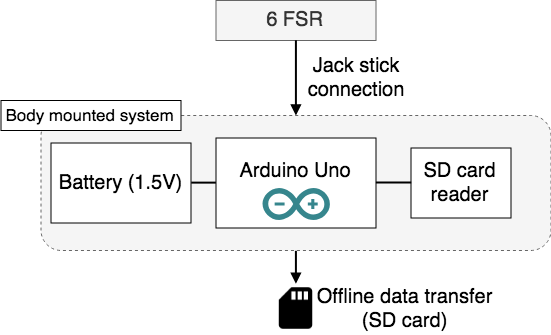
\includegraphics[width=.6\textwidth]{figures/circuitBoardSetup}
%	\caption{The setup of the Arduino-setup used for data collection from the FSRs on the feet. Collected data is saved on an SD card and transferred offline to be processed on a computer with MATLAB.}
%	\label{fig:circuitBoardSetup}  %<--remember LABEL!
%\end{figure}

The system setup as a whole for both the gyroscope and FSR parts can be seen illustrated as a block diagram on \figref{fig:heleSystemSetup}.

\begin{figure}[H]
	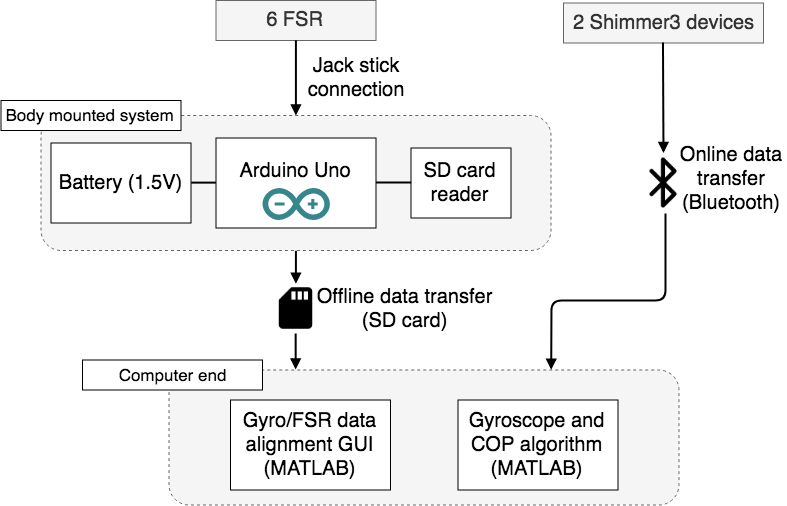
\includegraphics[width=.6\textwidth]{figures/heleSystemSetup}
	\caption{Block diagram of the system. The left side is of the pressure sensing part utilizing the FSRs. On the right side is the Shimmer3 devices (gyroscopes). All data is collected and processed on a computer using MATLAB.}
	\label{fig:heleSystemSetup}  %<--remember LABEL!
\end{figure}




\section{Data Acquisition}

During data acquisition the subjects will be wearing the instruments presented earlier in \secref{methods:instrumentation}. The Shimmer3 device will be placed lateral under the knees of the subject.

The FSRs will be placed on the sole of each foot of the subject. One FSR 406 is placed under the heel and two FSR 402 sensors are placed under the front of the foot at the lateral and medial part of the anterior eminence of the sole. The Arduino-setup will be placed at the lower back of the subject and handle data collection. Collected data will be stored on an SD card for later offline analysis with MATLAB. An illustration of device placement on a subject can be seen in \figref{fig:bodySysSetup}.

%% SENSOR BAIT ALERT:
%jeg har skrevet at vi placere en FSR 406 (den store firkant sensor) under hælen. den skal sidde "bag" lilletåen.
%sensor bait tekst flyttet til bNEWSystemTest.tex

\begin{figure}[H]
	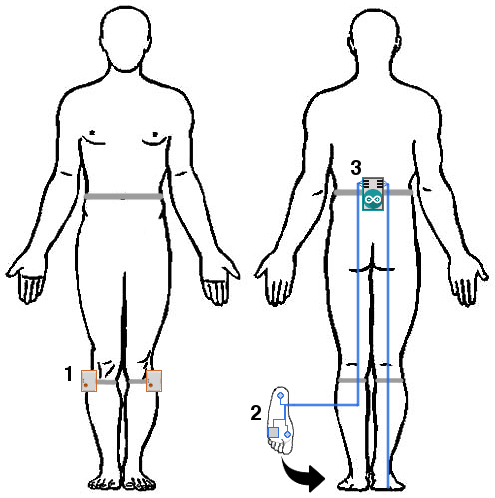
\includegraphics[width=.6\textwidth]{figures/bodySysSetup}
	\caption{The placement of the Shimmer3 IMU devices, Arduino-setup and FSRs on a test subject.}
	\label{fig:bodySysSetup}  %<--remember LABEL!
\end{figure}

Data acquisition from both the FSR sensors and the Shimmer3 devices are set to have a sample frequency of 100Hz. The sample rate is decided to be the same so it is possible to match the two data streams to each other, so it is possible to compare measured pressure forces under the feet while matching it to movement of the body. A simple graphical user interface (GUI) have been developed to match the data. This manual approach is favourable for this project as it were determined that it would be more time consuming to develop an algorithm to automatically match data streams. It would also go beyond the scope for the project.





All data is collected in MATLAB and organized into matrices. then something happens about calculating center of balance and maybe some rotational speed and something. 

Data acquisition from the Shimmer devices are handled by Bluetooth between the Shimmer devices and MATLAB. Sample frequency over 9000. Data is organized into a matrix, because that is the smart thing to do, when doing things in MATLAB.





we record stuff with the shimmers bluetooth directly to matlab and some jacksticks from the FSR's and save force data to an sd card which we put in matlab and organize it all into one matrix where we can do some math on. 

so far there might not be any filtering of any of the data









%bNEWSystemTest
%test
\section{System test}
This section covers the test of the system, prior to conducting the experiment for the project. 

\subsection{Method of test for gyroscopes}
The authors assess that a test of the gyroscopes is not necessary, as the Shimmer3 devices will be calibrated using the built in function of Shimmer Sensing’s program, Consensys, to ensure the devices are working as expected.

%til test af gyro/accel kan vi gøre som paul foreslog og filme personen imens de drejer rundt eller noget, hvor vi kan synkronisere film med gyro/accel målinger og se at der sker udsving på samme tidspunkt som personen drejer/bevæger sig. Det kan self ikke være med i rapporten men vi kan vise det til eksamen. 


\subsection{Method of test for Force Sensitive Resistors}
The FSRs will be tested by placing a 1kg weight covering a surface area of 1$cm^{2}$ applied in the middle of both types of FSRs. This is done to test if any of the sensors are broken or deviate compared to the other FSRs. %mean result of the test.

%retfærdigøre at vi brugere sensore der "kun" kan måle så lidt tryk til at måle under folk som vejer +50 kg. Sikkert noget med at simon har sat modstande i systemet som øger sensorernes måling af tryk påvirkning. 

\subsection{Test  results for Force Sensitive Resistors}
A weight of 1kg were applied to each FSR in order from FSR channel 1 to 6. The weight were applied for approximately five seconds to each FSR in the middle of the sensor area. Results of the test of the FSRs is shown in \figref{fig:FSRTestPlot1kg}.

\begin{figure}[H]
	\includegraphics[width=.6\textwidth]{figures/FSRTestPlot1kg}
	\caption{The result of the test of the six FSRs.}
	\label{fig:FSRTestPlot1kg}  %<--remember LABEL!
\end{figure}

As it can be seen from the results none of the sensors are broken, however FSR number 3 (FSR#3), located at the heel of the right foot, returns a lower resistance when applied a 1kg weight compared to the other FSRs. 

%Tell the truth.
%The authors learned too late in the work period that one of the FSRs were returning resistance varying from the other FSRs. This was not anticipated and no replacement had been ordered. However, the authors hope/judge/evaluate that the FSR will not affect the data processing the calculations of Centre of Pressure (COP) too much.

%tell the lie
%During continuous testing of the system during development the authors experienced damage to one of the FSRs, and are at this point in the work, unable to obtain a replacement. However, as this project is mainly to function as a proof of concept work, the authors determine that one sensor should not have too much of an effect.

%tell the something-in-between
This could prove a problem if data were to be compared between individual FSRs, however the output for each FSR sensors will be used for estimation of a point for the subjects COP, which will be used to compare COP between subjects. Thus, the FSR#3 measurement will not have an effect as long as FSR#3 have the same deviance for every subject. 



\subsection{System test}
The system as a whole will be tested with a walk sequence. The sequence will involve periods of no movement, movement by walking and turning and a light jump to mark the beginning and end of the sequence. The test walk sequence is as follows:
\vspace{-0.6cm}
\begin{itemize}
	\item 5 second pause
	\vspace{-0.3cm}
	\item Light jump
	\vspace{-0.3cm}
	\item 5 second pause
	\vspace{-0.3cm}
	\item Walk five steps
	\vspace{-0.3cm}
	\item 180 degree turn
	\vspace{-0.3cm}
	\item Walk five steps
	\vspace{-0.3cm}
	\item 5 second pause
	\vspace{-0.3cm}
	\item Light jump
	\vspace{-0.3cm}
	\item 5 second pause
\end{itemize}
\vspace{-0.4cm}
%Test walk sequence: Wait 3 sec. light jump. wait 1 sec. walk 5 steps. 180 turn. walk 5 steps. 90 turn right. wait. 90 turn right. wait. quick 180. wait quick 180. wait 1. light jump. wait 3 sec. 
Following the system test the acquired data will be qualitatively evaluated to ensure everything works as intended. 

\subsection{Test results for System test}
%Everything was fine. maybe.
Result of the system test as a whole were successful, despite lower readings from FSR#3. Acquired data were plotted for each FSR channel so the recorded output could be viewed alongside a video recording of the test walk sequence. At each step FSRs were reacting and returning values consistent with what would be expected when pressure were either applied to or removed from the sensors. 
It is concluded that, as the lower resistance returned from FSR#3 will be consistent for all data collection, the \textit{"error"} will be present in each data set and therefore should not have any effect on comparison between subjects. 

%not necessary 
%A problem occurred with the FSR 406 placed under the heel of the subject during the system test . When weight was applied to the sensor it would measure the highest possible force the sensor can measure, and no useful data could be collected from the sensor. It was evaluated why this happened and discovered that because the FSR 406 covers a larger area and were placed at the heel it would be affected by more force when a subject stood on it. As the distribution of pressure is higher at the heel compared to anywhere else under the foot while standing, it makes sense that the FSR 406 would be overloaded \cite{Hessert2005}. To account for this, the FSR 402 placed at the lateral side of the feet where switched with the FSR 406 at the heel. As the FSR 402 covers a smaller area they would not be overloaded as easily as the FSR 406. As a result the FSR 406 is now placed at the lateral side of the eminence of the sole, and one FSR 402 is placed at the heel. The new placement of FSR sensors can be seen in \figref{fig:soleSensorPlacement}.
%With the new placement of the FSR’s the system functions as intended and is ready for the experiment. 

\section{Protocol}
%Pinan Nidan Kata sequence with force and gyroscopic sensors
\subsection{Aim}
The experiment aims to measure the ground reaction forces during the performance of the karate kata Pinan Nidan. At the same time gyroscopic sensors will measure the rotational forces of the legs for later use in data analysis.

\subsection{Design}
\subsubsection{Before the experiment}
\begin{itemize}
\item The data file “Data.txt” on the SD card for the Arduino will be emptied and the SD card will then be placed in the Arduino-setup. 
\item Subjects have knowledge and various amounts of experience with the kata Pinan Nidan prior to the experiment. No subject needs instruction of performance of the kata.
\end{itemize}

\subsubsection{Initial part}
\begin{enumerate}
\item The person responsible for the test will mount the force sensors underneath the feet of the subject according to the labelling on the sensors. These sensors will be placed as following on both feet:
\begin{itemize}
$\bullet$ One FSR406 sensor on the lateral eminence of the sole \\
$\bullet$ One FSR402 sensor on the medial eminence of the sole \\
$\bullet$ One FSR402 sensor at the heel \\
\end{itemize}
\item The distance between the sensors will be measured for later use. 
\item 1 Shimmer3 device (gyroscopes) will be mounted lateral distal to the knee. One sensor on each leg.
\item The Arduino-setup will be mounted around the waist, and the system will be placed at the lower back.
\item Elastic straps will be mounted right above the knee to ensure the cables for the force sensors stays in place, and to mount the Shimmer3 devices.
\item The force sensors will be plugged into the Arduino-setup according to the numbering on both the system and the sensor cables.
\item Shimmer3 devices will be connected to MATLAB.
\item The subject will practice one round of Pinan Nidan to warm up.
\item The subject stands ready to begin performing Pinan Nidan with recordings.
\end{enumerate}

\subsubsection{Data acquisition part}
\begin{enumerate}
\item Recording from the Shimmer3 devices will be initiated in MATLAB.
\item The Arduino system will be powered up and recording started by pressing the designated “Record” button until the red LED lights up.
\item Subject will be asked to stand still for 5 seconds then do a small jump, stand still for 5 seconds, do another small jump and then stand still for 5 seconds before moving on.
\item After this initial movement, the subject will be asked to perform the Pinan Nidan.
\item When the subject is done with the Pinan Nidan, they will be asked to perform a 5 second pause, small jump and 5 second pause again.
\item The recording is stopped by pressing the “Record” button until the red LED turns off. The Arduino-setup will be shut off and the microSD card removed from the setup to extract the data to a computer.
\item After data is transferred to the computer, the microSD card is inserted to the Arduino-setup, and the process continues from step 1 in “Data acquisition part”.
\end{enumerate}

The subject will perform Pinan Nidan four times in total, one for practice and three were data is acquired.

\subsubsection{Removal of the system}
\begin{enumerate}
\item After the data acquisition the subject will be asked to stand still and the Shimmer datastream will be stopped. 
\item At the same time the “Record” button on the Arduino will be pressed until the red LED turns of. 
\item The Arduino-system will be turned off and all the sensors and the Arduino will be removed from the subject.
\end{enumerate}

\subsection{Participants and statistical considerations}
The included three participants are selected based on their experience with the kata Pinan Nidan. This includes a master (+30 years of karate experience), intermediate (3-5 years of karate experience) and novice (less than 1 year of karate experience) The number of participants is chosen as the study doesn’t aim to find a statistical significant difference between the subjects, but rather aim to examine if there’s a way to determine the stability of the subjects during the Pinan Nidan.

The time for the experiment will be 45-60 minutes.


%\chapter{Results} \label{chap:Results}


%\chapter{Discussion} \label{chap:Discussion}


%\chapter{Conclusion} \label{chap:Conclusion}




\clearpage
%\begin{multicols}{2}
	
\urlstyle{same}
\printbibliography			% to bibliography: "compile" -> Tools -> Commands -> "Bibtex" -> "compile/build"
\clearpage
%\end{multicols}


%\cleardoublepage
% BILAG
%\begin{appendices}
%	\chapter{Appendices}
%
%\end{appendices}


\end{document}
